\documentclass[12pt]{article}
\usepackage{amsmath, amssymb, amsthm, tikz, pgfplots}
\usepackage{geometry, enumitem, mdframed, array, xcolor}
% \usepackage{nicematrix, systeme} % Packages not available
\geometry{margin=1in}

% Custom environments
\newtheorem{definition}{Definition}
\newtheorem{theorem}{Theorem}
\newtheorem{method}{Method}
\newtheorem{example}{Example}
\newmdenv[linecolor=blue,linewidth=2pt]{keypoint}
\newmdenv[linecolor=red,linewidth=2pt]{warning}
\newmdenv[linecolor=green,linewidth=2pt]{insight}
\newmdenv[linecolor=purple,linewidth=2pt]{examtip}
\newmdenv[linecolor=orange,linewidth=2pt]{eigenvalue}

\title{ODE Lesson 30: Constant Coefficient Systems - Distinct Eigenvalues}
\author{ODE 1 - Prof. Adi Ditkowski}
\date{}

\begin{document}
\maketitle

\section{Theory of Linear Systems}

\begin{definition}[Linear System with Constant Coefficients]
A system of linear ODEs with constant coefficients has the form:
\begin{equation}
\mathbf{x}'(t) = A\mathbf{x}(t)
\end{equation}
where $\mathbf{x}(t) = [x_{1}(t), x_{2}(t), \ldots, x_{n}(t)]^{T}$ and $A$ is an $n \times n$ constant matrix.
\end{definition}

\begin{theorem}[Fundamental Solution Structure]
If $\lambda$ is an eigenvalue of $A$ with eigenvector $\mathbf{v}$, then $\mathbf{x}(t) = e^{\lambda t}\mathbf{v}$ is a solution to $\mathbf{x}' = A\mathbf{x}$.
\end{theorem}

\begin{proof}
Direct verification:
\[\frac{d}{dt}(e^{\lambda t}\mathbf{v}) = \lambda e^{\lambda t}\mathbf{v} = e^{\lambda t}(\lambda \mathbf{v}) = e^{\lambda t}(A\mathbf{v}) = A(e^{\lambda t}\mathbf{v})\]
\end{proof}

\begin{eigenvalue}
\textbf{Eigenvalue Computation Algorithm:}
\begin{enumerate}
\item Form the characteristic polynomial: $p(\lambda) = \det(A - \lambda I)$
\item Expand the determinant (cofactor expansion for $3 \times 3$ or larger)
\item Solve $p(\lambda) = 0$ for eigenvalues $\lambda_{1}, \lambda_{2}, \ldots, \lambda_{n}$
\item For each $\lambda_{i}$, solve $(A - \lambda_{i} I)\mathbf{v} = \mathbf{0}$ for eigenvector $\mathbf{v}_{i}$
\end{enumerate}
\end{eigenvalue}

\begin{theorem}[General Solution for Distinct Eigenvalues]
If $A$ has $n$ distinct eigenvalues $\lambda_{1}, \ldots, \lambda_{n}$ with corresponding eigenvectors $\mathbf{v}_{1}, \ldots, \mathbf{v}_{n}$, then the general solution is:
\begin{equation}
\mathbf{x}(t) = c_{1} e^{\lambda_{1} t}\mathbf{v}_{1} + c_{2} e^{\lambda_{2} t}\mathbf{v}_{2} + \cdots + c_{n} e^{\lambda_{n} t}\mathbf{v}_{n}
\end{equation}
\end{theorem}

\begin{keypoint}
\textbf{Matrix Diagonalization Perspective:}\\
If $P = [\mathbf{v}_{1} | \mathbf{v}_{2} | \cdots | \mathbf{v}_{n}]$ and $D = \text{diag}(\lambda_{1}, \ldots, \lambda_{n})$, then:
\begin{itemize}
\item $A = PDP^{-1}$
\item Solution: $\mathbf{x}(t) = Pe^{Dt}P^{-1}\mathbf{x}_{0}$
\item Where $e^{Dt} = \text{diag}(e^{\lambda_{1} t}, \ldots, e^{\lambda_{n} t})$
\end{itemize}
\end{keypoint}

\section{Solution Method Step-by-Step}

\begin{method}[Complete Solution Algorithm]
Given $\mathbf{x}' = A\mathbf{x}$ with $\mathbf{x}(0) = \mathbf{x}_{0}$:

\textbf{Step 1: Find Eigenvalues}
\begin{itemize}
\item Compute $\det(A - \lambda I) = 0$
\item For $2 \times 2$: $\det\begin{pmatrix} a_{11}-\lambda & a_{12} \\ a_{21} & a_{22}-\lambda \end{pmatrix} = 0$
\item Expand: $\lambda^{2} - \text{tr}(A)\lambda + \det(A) = 0$
\end{itemize}

\textbf{Step 2: Find Eigenvectors}
\begin{itemize}
\item For each $\lambda_{i}$, solve $(A - \lambda_{i} I)\mathbf{v} = \mathbf{0}$
\item Row reduce to find null space
\item Choose convenient basis vector
\end{itemize}

\textbf{Step 3: Form General Solution}
\begin{itemize}
\item Write $\mathbf{x}(t) = \sum_{i=1}^{n} c_{i} e^{\lambda_{i} t}\mathbf{v}_{i}$
\end{itemize}

\textbf{Step 4: Apply Initial Conditions}
\begin{itemize}
\item Set $t = 0$: $\mathbf{x}_{0} = \sum_{i=1}^{n} c_{i} \mathbf{v}_{i}$
\item Solve linear system for $c_{1}, \ldots, c_{n}$
\end{itemize}
\end{method}

\begin{example}[Complete $2\times2$ System]
Solve $\mathbf{x}' = \begin{pmatrix} 4 & 2 \\ 3 & -1 \end{pmatrix}\mathbf{x}$ with $\mathbf{x}(0) = \begin{pmatrix} 1 \\ 2 \end{pmatrix}$

\textbf{Solution:}
\begin{enumerate}
\item \textbf{Eigenvalues:}
\[\det(A - \lambda I) = \det\begin{pmatrix} 4-\lambda & 2 \\ 3 & -1-\lambda \end{pmatrix} = (4-\lambda)(-1-\lambda) - 6\]
\[= -4 - 4\lambda + \lambda + \lambda^{2} - 6 = \lambda^{2} - 3\lambda - 10 = 0\]
\[(\lambda - 5)(\lambda + 2) = 0 \implies \lambda_{1} = 5, \lambda_{2} = -2\]

\item \textbf{Eigenvectors:}

For $\lambda_{1} = 5$:
\[(A - 5I)\mathbf{v} = \begin{pmatrix} -1 & 2 \\ 3 & -6 \end{pmatrix}\begin{pmatrix} v_{1} \\ v_{2} \end{pmatrix} = \begin{pmatrix} 0 \\ 0 \end{pmatrix}\]
Row 1: $-v_{1} + 2v_{2} = 0 \implies v_{1} = 2v_{2}$. Choose $v_{2} = 1$: $\mathbf{v}_{1} = \begin{pmatrix} 2 \\ 1 \end{pmatrix}$

For $\lambda_{2} = -2$:
\[(A + 2I)\mathbf{v} = \begin{pmatrix} 6 & 2 \\ 3 & 1 \end{pmatrix}\begin{pmatrix} v_{1} \\ v_{2} \end{pmatrix} = \begin{pmatrix} 0 \\ 0 \end{pmatrix}\]
Row 2: $3v_{1} + v_{2} = 0 \implies v_{2} = -3v_{1}$. Choose $v_{1} = 1$: $\mathbf{v}_{2} = \begin{pmatrix} 1 \\ -3 \end{pmatrix}$

\item \textbf{General Solution:}
\[\mathbf{x}(t) = c_{1} e^{5t}\begin{pmatrix} 2 \\ 1 \end{pmatrix} + c_{2} e^{-2t}\begin{pmatrix} 1 \\ -3 \end{pmatrix}\]

\item \textbf{Initial Conditions:}
\[\begin{pmatrix} 1 \\ 2 \end{pmatrix} = c_{1}\begin{pmatrix} 2 \\ 1 \end{pmatrix} + c_{2}\begin{pmatrix} 1 \\ -3 \end{pmatrix}\]
System: $2c_{1} + c_{2} = 1$ and $c_{1} - 3c_{2} = 2$

From equation 2: $c_{1} = 2 + 3c_{2}$. Substitute into equation 1:
\[2(2 + 3c_{2}) + c_{2} = 1 \implies 4 + 7c_{2} = 1 \implies c_{2} = -\frac{3}{7}\]
\[c_{1} = 2 + 3(-\frac{3}{7}) = 2 - \frac{9}{7} = \frac{5}{7}\]

\item \textbf{Final Solution:}
\[\mathbf{x}(t) = \frac{5}{7}e^{5t}\begin{pmatrix} 2 \\ 1 \end{pmatrix} - \frac{3}{7}e^{-2t}\begin{pmatrix} 1 \\ -3 \end{pmatrix}\]
\end{enumerate}
\end{example}

\begin{warning}
\textbf{Common Errors:}
\begin{itemize}
\item Forgetting that eigenvectors are determined up to scalar multiplication
\item Sign errors when computing $\det(A - \lambda I)$
\item Not verifying eigenvectors: always check $A\mathbf{v} = \lambda\mathbf{v}$
\item Arithmetic mistakes in the linear system for constants
\end{itemize}
\end{warning}

\begin{insight}
\textbf{Solution Behavior from Eigenvalues:}
\begin{itemize}
\item All $\lambda_{i} < 0$: Stable node (all solutions $\to \mathbf{0}$)
\item All $\lambda_{i} > 0$: Unstable node (all solutions grow)
\item Mixed signs: Saddle point
\item $\lambda_{i} = 0$: Non-isolated equilibrium (degenerate)
\end{itemize}
\end{insight}

\begin{examtip}
Prof. Ditkowski's exams typically include:
\begin{itemize}
\item One $2\times2$ system (always)
\item Possibly one $3\times3$ system
\item Initial value problems (60\% of system problems)
\item Questions about stability based on eigenvalues
\item Verification of solutions
\end{itemize}
\end{examtip}

\section{Phase Portrait Connection}

The eigenvalues and eigenvectors completely determine the phase portrait:
\begin{itemize}
\item Eigenvectors give the principal directions
\item Eigenvalues give the behavior along each direction
\item Trajectories are tangent to eigenvector directions at the origin
\end{itemize}

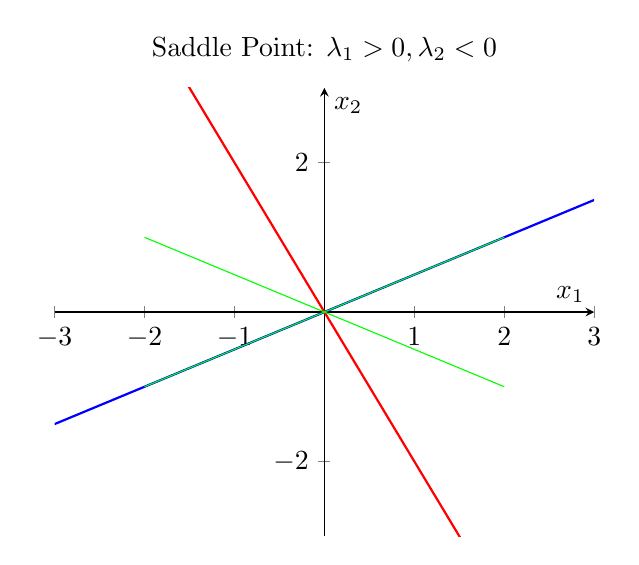
\begin{tikzpicture}
\begin{axis}[
    axis lines = center,
    xlabel = $x_{1}$,
    ylabel = $x_{2}$,
    xmin=-3, xmax=3,
    ymin=-3, ymax=3,
    title={Saddle Point: $\lambda_{1} > 0, \lambda_{2} < 0$}
]
% Eigenvector directions
\addplot[domain=-3:3, samples=2, thick, blue] {0.5*x};
\addplot[domain=-3:3, samples=2, thick, red] {-2*x};
% Sample trajectories (hyperbolic curves)
\addplot[domain=-2:2, samples=50, green, smooth] {x/2};
\addplot[domain=-2:2, samples=50, green, smooth] {-x/2};
\end{axis}
\end{tikzpicture}

\end{document}